\chapter*{Appendix A - Algorithms for Evaluation}
\addcontentsline{toc}{chapter}{Appendix A}

\begin{algorithm}
	\caption{Update Algorithm of EvalWriter}
	\label{alg:upd}
	Get current $dist$ and $t_{sim}$ from environment $\epsilon$ and save it
	
	\If{$e = 1$}{
		Add pose of the drone from $\epsilon$ to pathplotter
		}
		
	\If{$t_{sim} = \frac{T}{2}$}{
		Save current $dist$ to matching set of distances
		}
		
	\If{$t_{sim} = T$}{
		Save current $dist$ to matching set of distances
	}
	
	\If{episode already reached goal and overshoot}{
		Save current $dist$ to overshoot set
	}
	
	Check if the episode succeeded in this time step
\end{algorithm}

\begin{algorithm}
	\caption{Evaluation Algorithm of EvalWriter}
	\label{alg:evalwriter}
	\KwIn{policy $\pi$}
	\KwOut{tupel ($\mu_r, \sigma_r$)}
	
	Get mean return $\mu_r$ and the std of the return $\sigma_r$ from $evaluate\_policy (\pi , \epsilon, e)$
	
	reset $\epsilon$ and receive $\daleth_t$
	
	\For{$j=0 \to \gimel$}{
		\Repeat{$done$}{
			Get action $a$ from $\pi$ with input $\daleth_t$
			
			Step $\epsilon$ and get the new observation $\daleth_t$, reward $r_t$, done signal $d$  and info
			
			Update EvalWriter
			
			\If{$d$}{
				Reset $\epsilon$
				}
		}
		\If{not $j = \gimel$}{
			Use Housekeeping of the EvalWriter class
			}
	}
	Close EvalWriter and $\epsilon$.
	
	\Return ($\mu_r, \sigma_r$)
	
\end{algorithm} 

\newpage

\chapter*{Appendix B - Flight \& Distance Data}
\addcontentsline{toc}{chapter}{Appendix B}

\begin{figure}[htp]
	\centering
	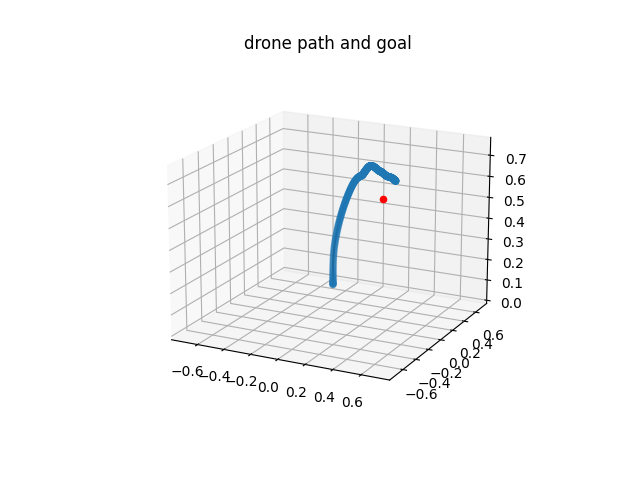
\includegraphics[width=0.6\linewidth]{figures/exampleflight1.png}
	\caption{Example of a flight with SAC policy on mode 2 within a radius of $0.5m$}
	\label{fig:flight0}
\end{figure}

\begin{figure}[htp]
	\centering
	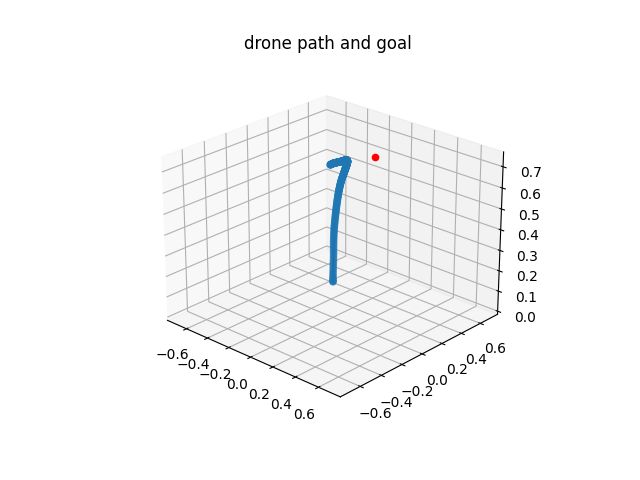
\includegraphics[width=0.6\linewidth]{figures/flight2.png}
	\caption{Example of a flight with SAC policy derived from LCL with $\delta = 0.4$ on mode 2 within a radius of $0.5m$}
	\label{fig:flight1}
\end{figure}

\begin{figure}[htp]
	\centering
	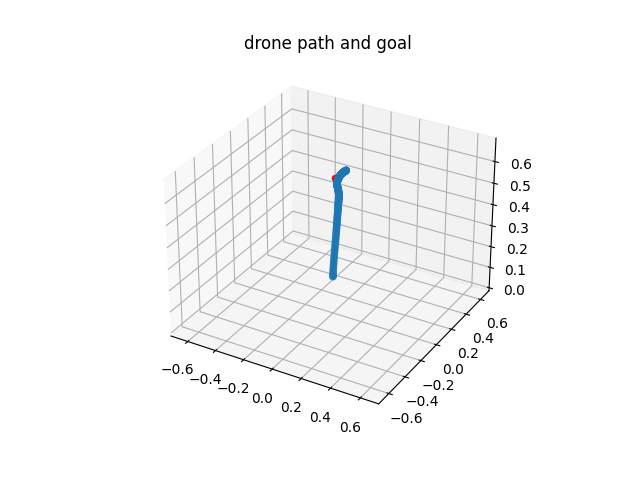
\includegraphics[width=0.6\linewidth]{figures/flight3.png}
	\caption{Example of a flight with SAC policy derived from LCL with $\delta = 0.2$ on mode 2 within a radius of $0.5m$}
	\label{fig:flight2}
\end{figure}

\begin{figure}[htp]
	\centering
	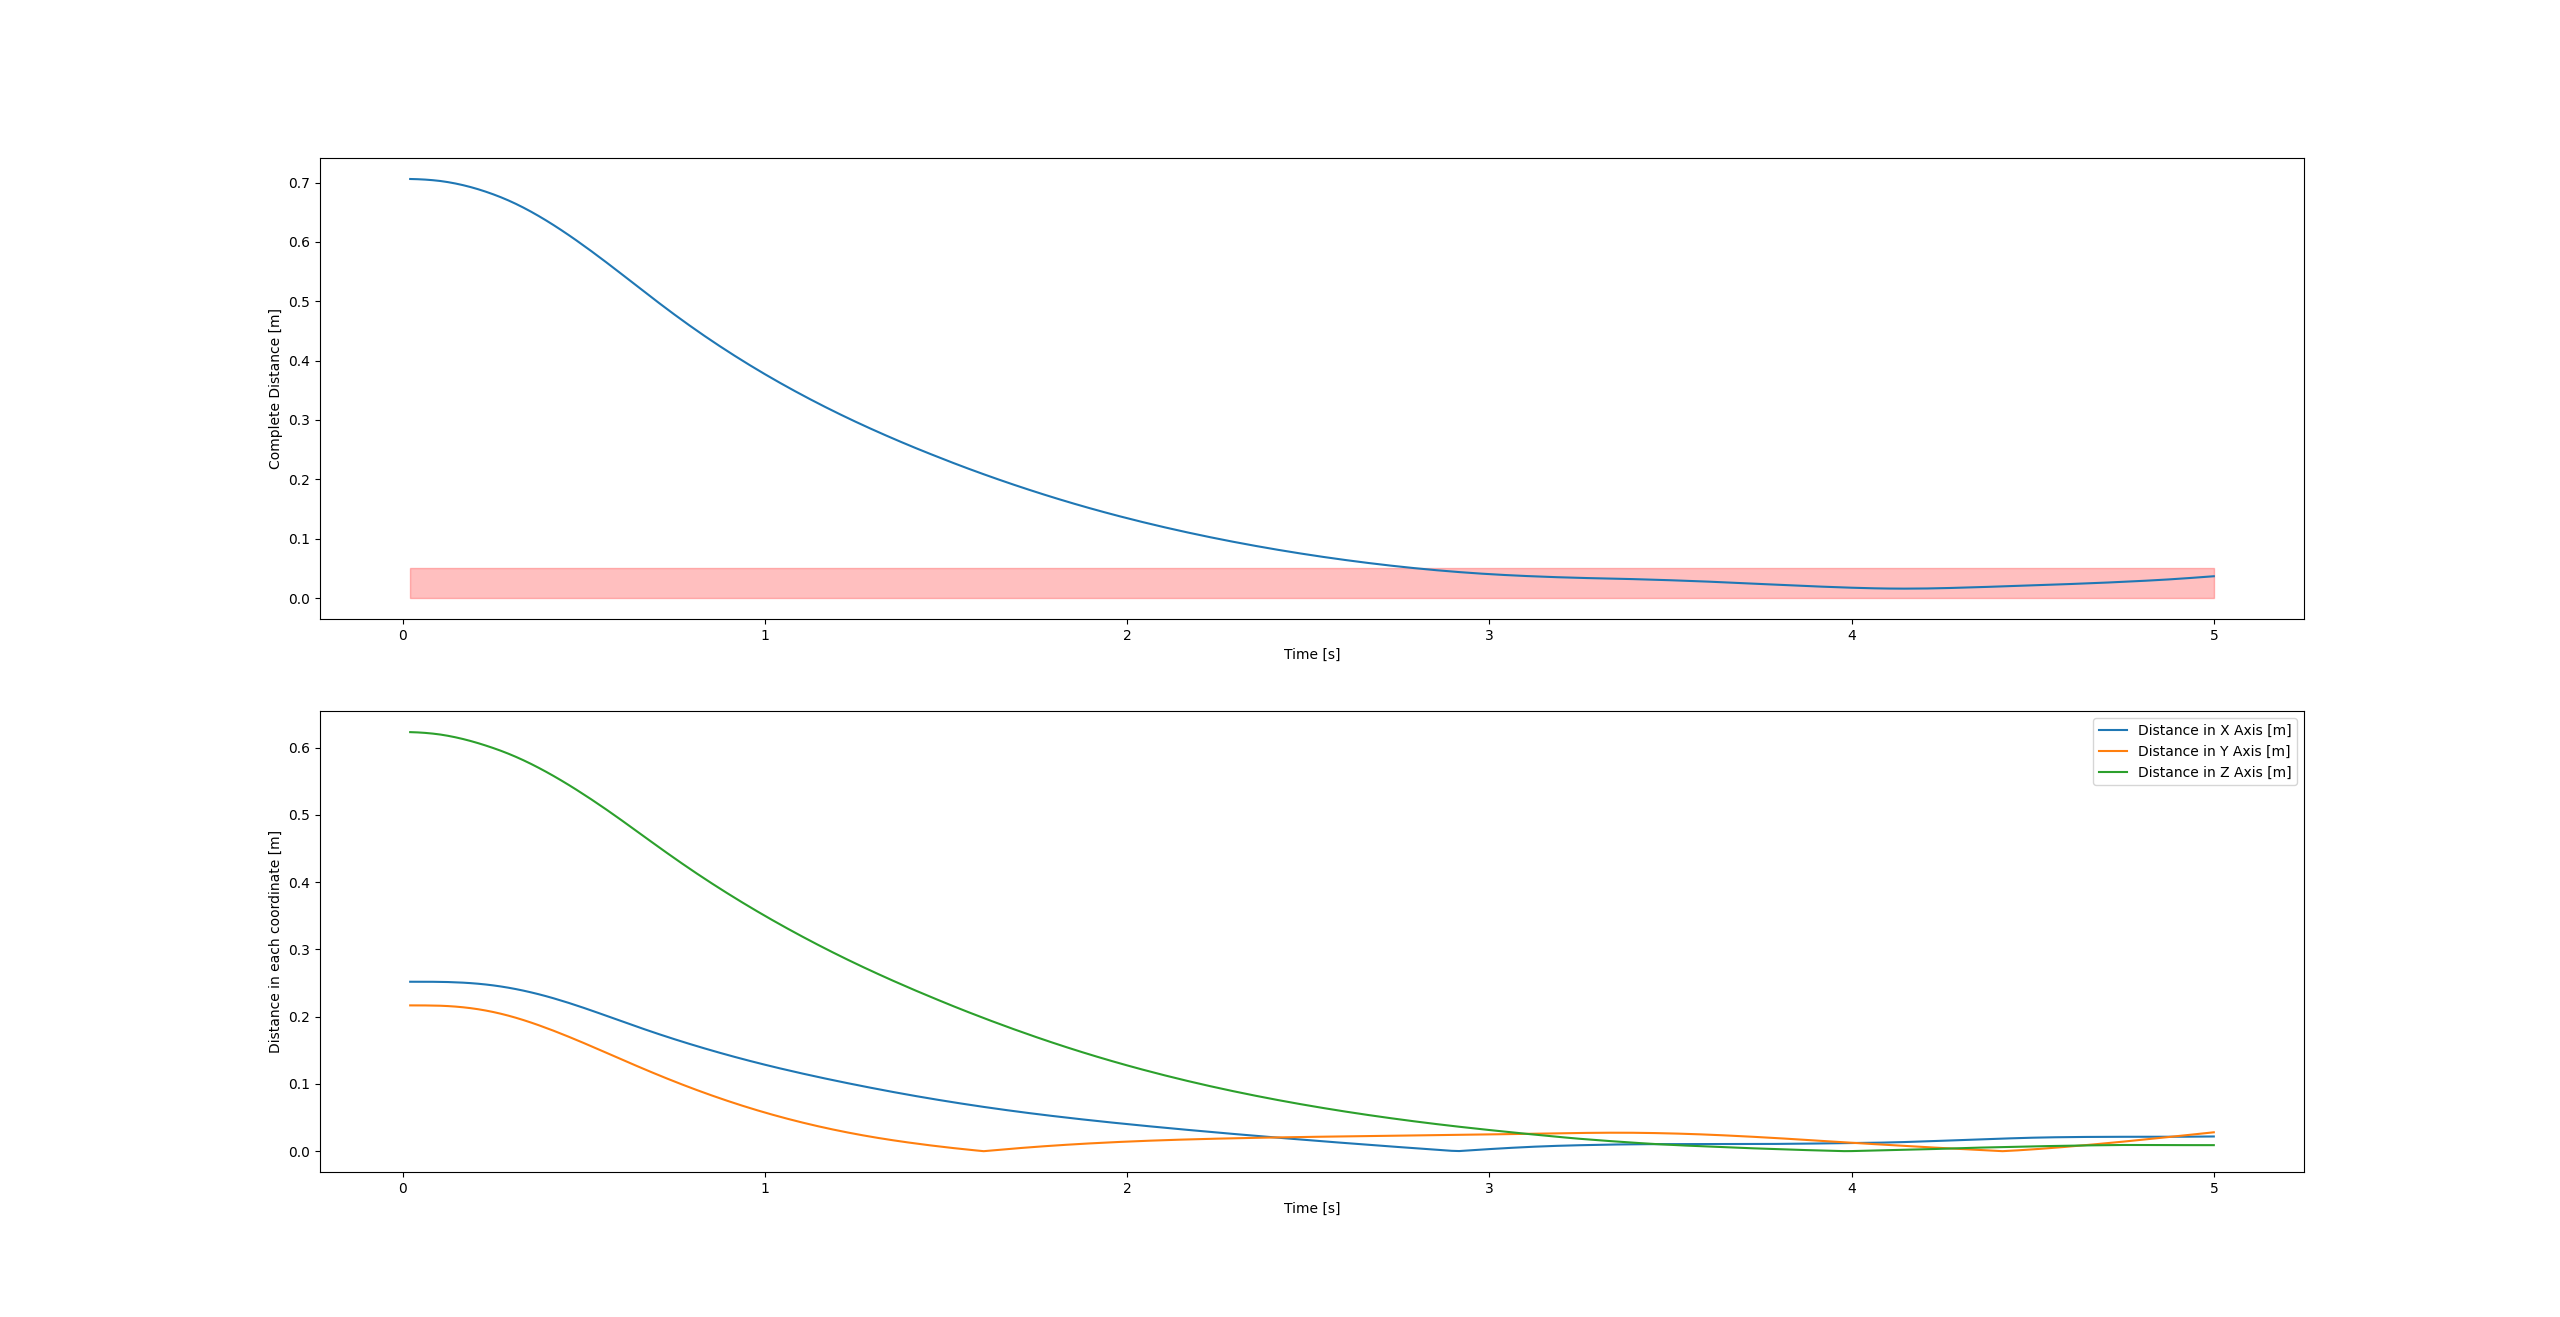
\includegraphics[width=\linewidth]{figures/flight4dist.png}
	\caption{Example of distances with SAC policy on mode 2 within a radius of $0.5m$}
	\label{fig:flight3}
\end{figure}

\begin{figure}[htp]
	\centering
	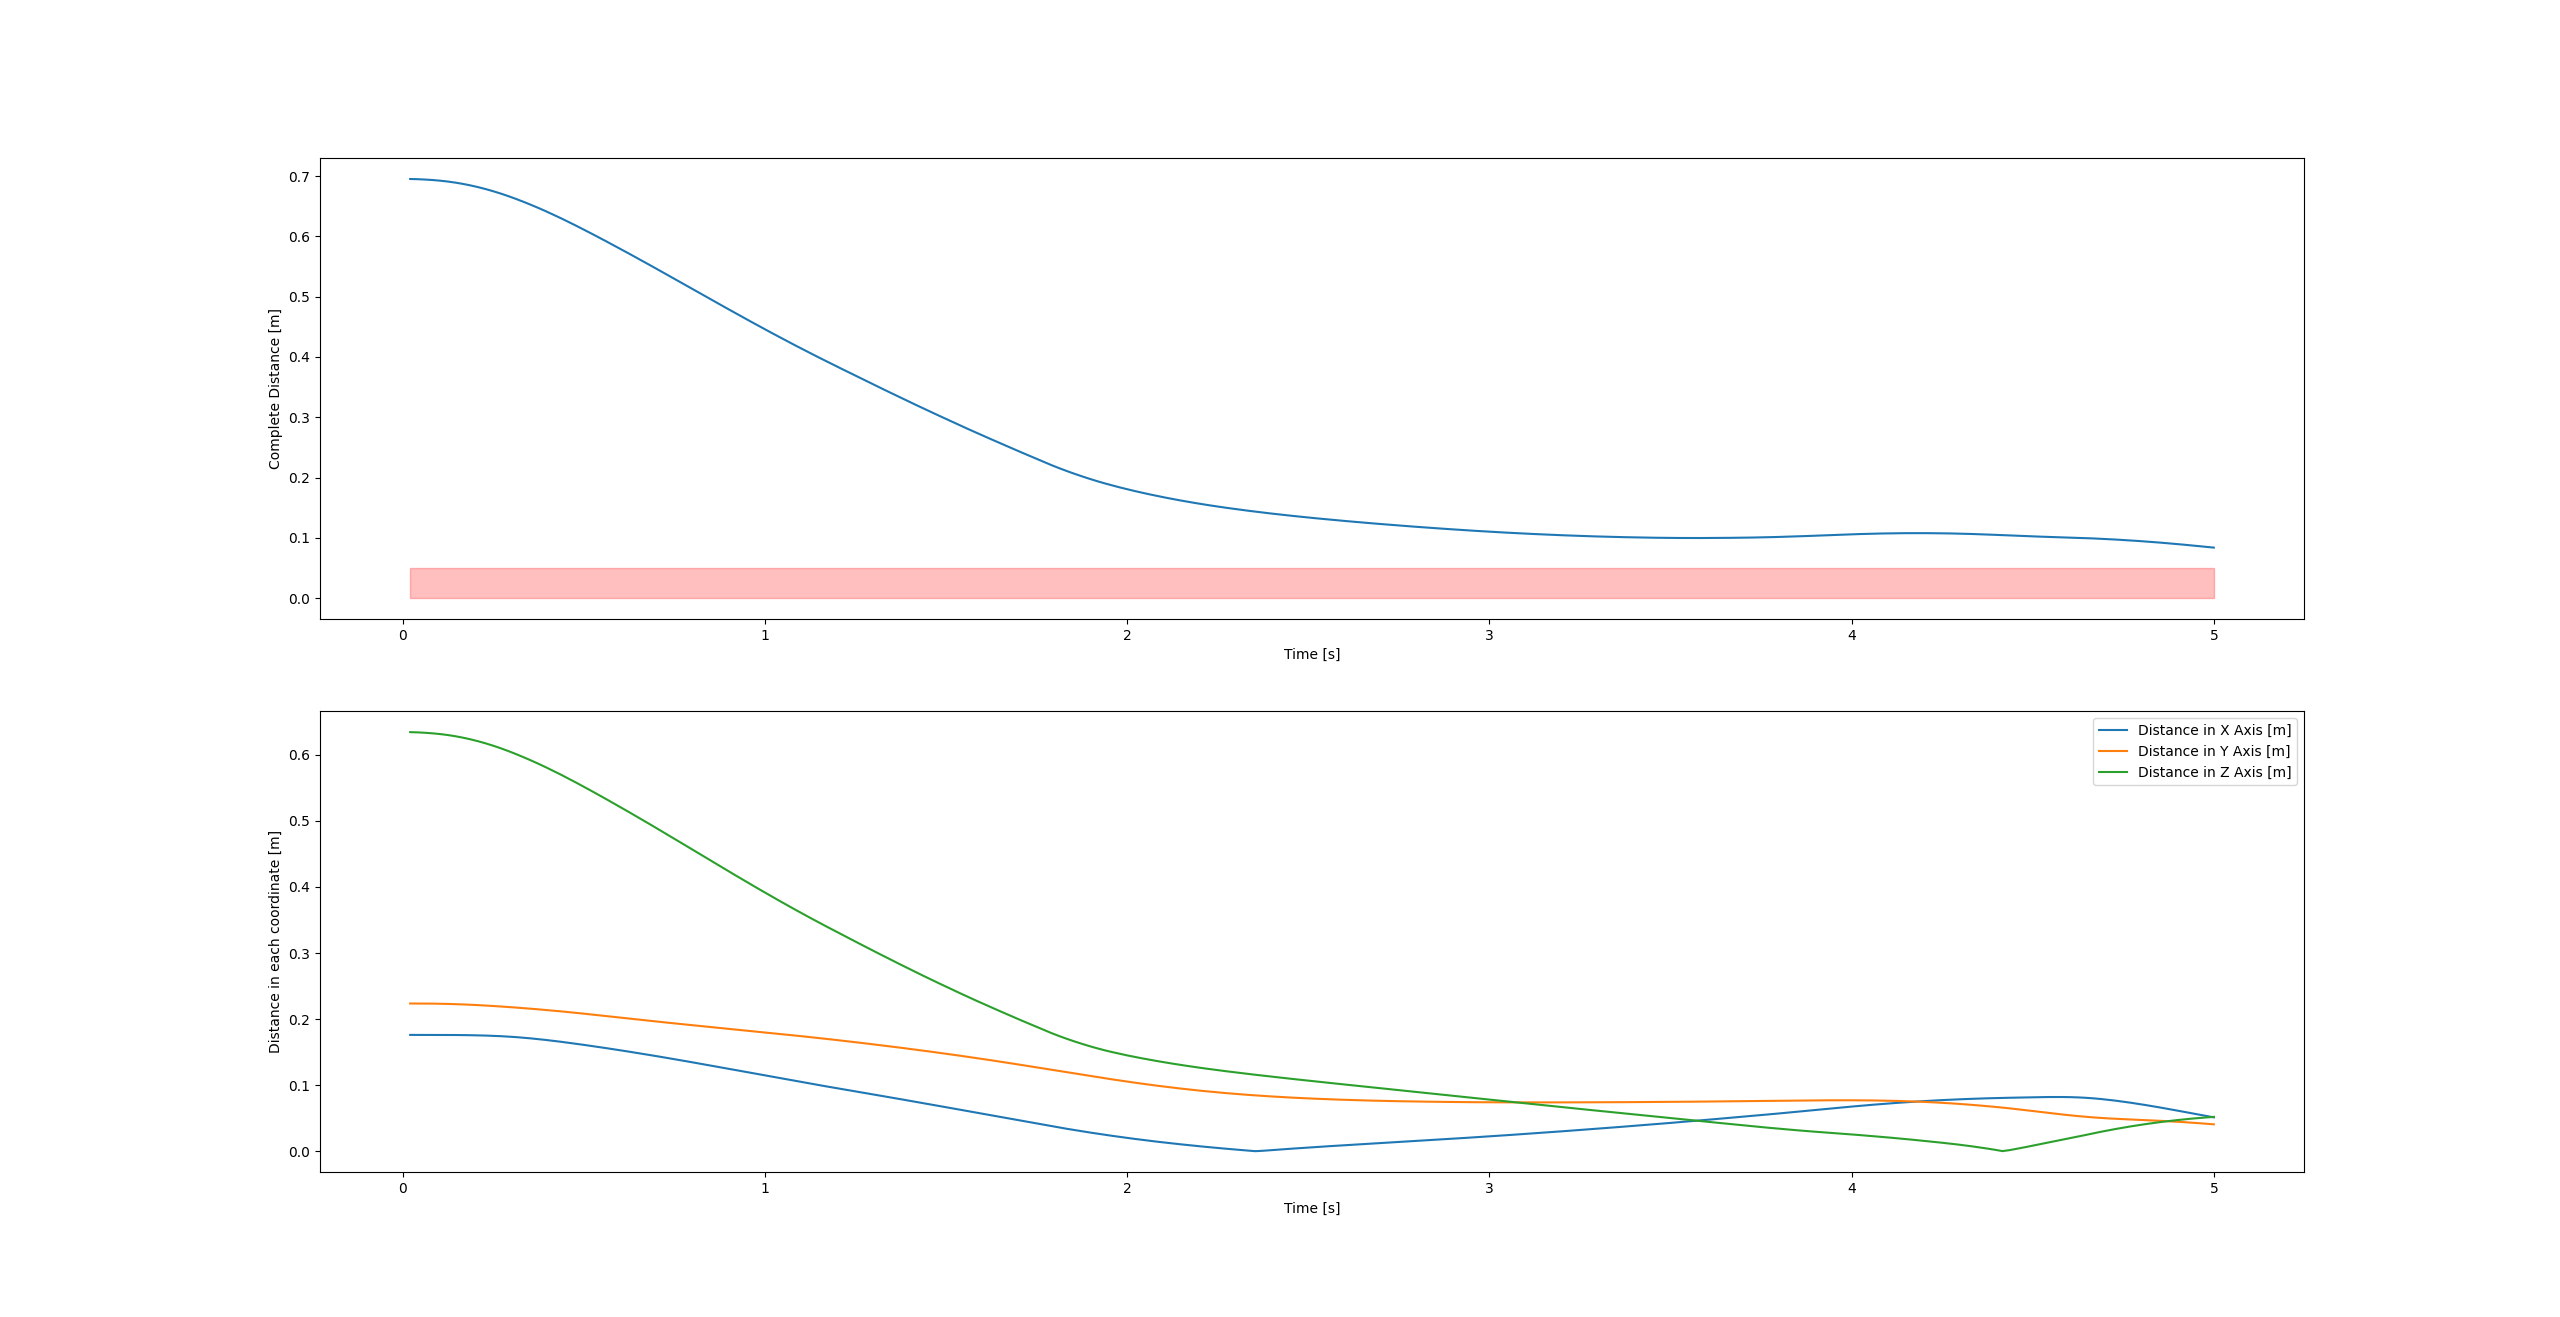
\includegraphics[width=\linewidth]{figures/flight5dist.png}
	\caption{Example of distances with SAC policy derived from LCL with $\delta = 0.4$ on mode 2 within a radius of $0.5m$}
	\label{fig:flight4}
\end{figure}

\begin{figure}[htp]
	\centering
	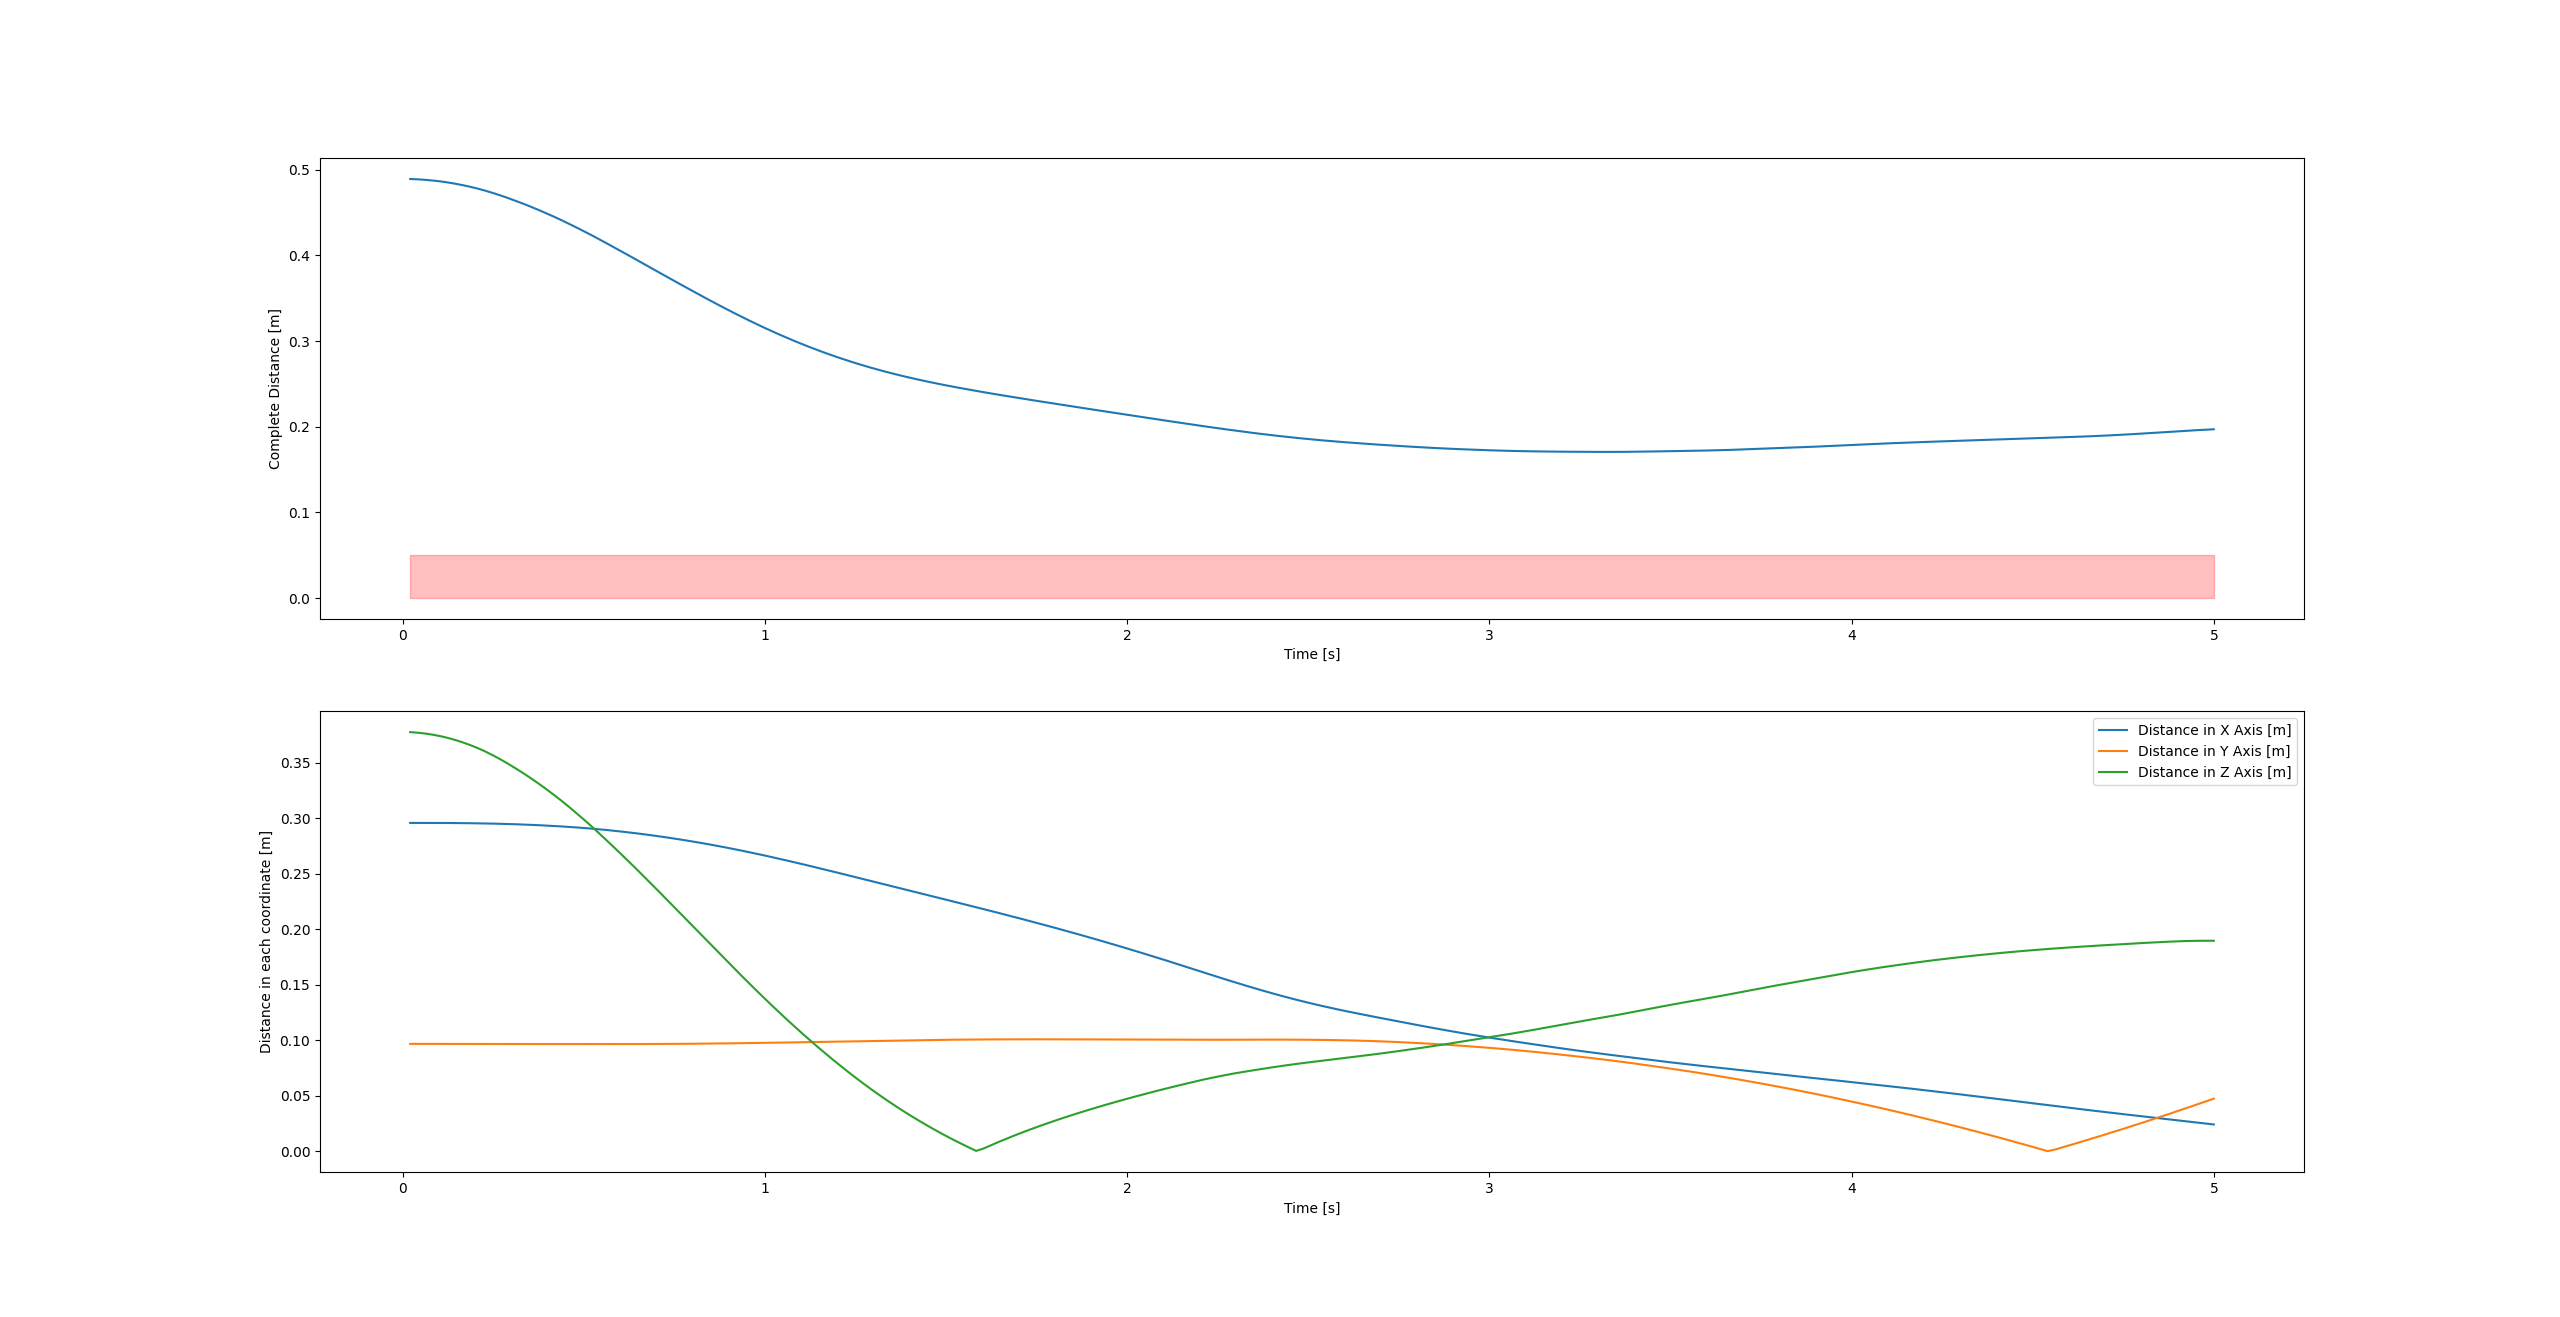
\includegraphics[width=\linewidth]{figures/flight6dist.png}
	\caption{Example of a distances with SAC policy derived from LCL with $\delta = 0.2$ on mode 2 within a radius of $0.5m$}
	\label{fig:flight5}
\end{figure}

\begin{figure}
	\centering
	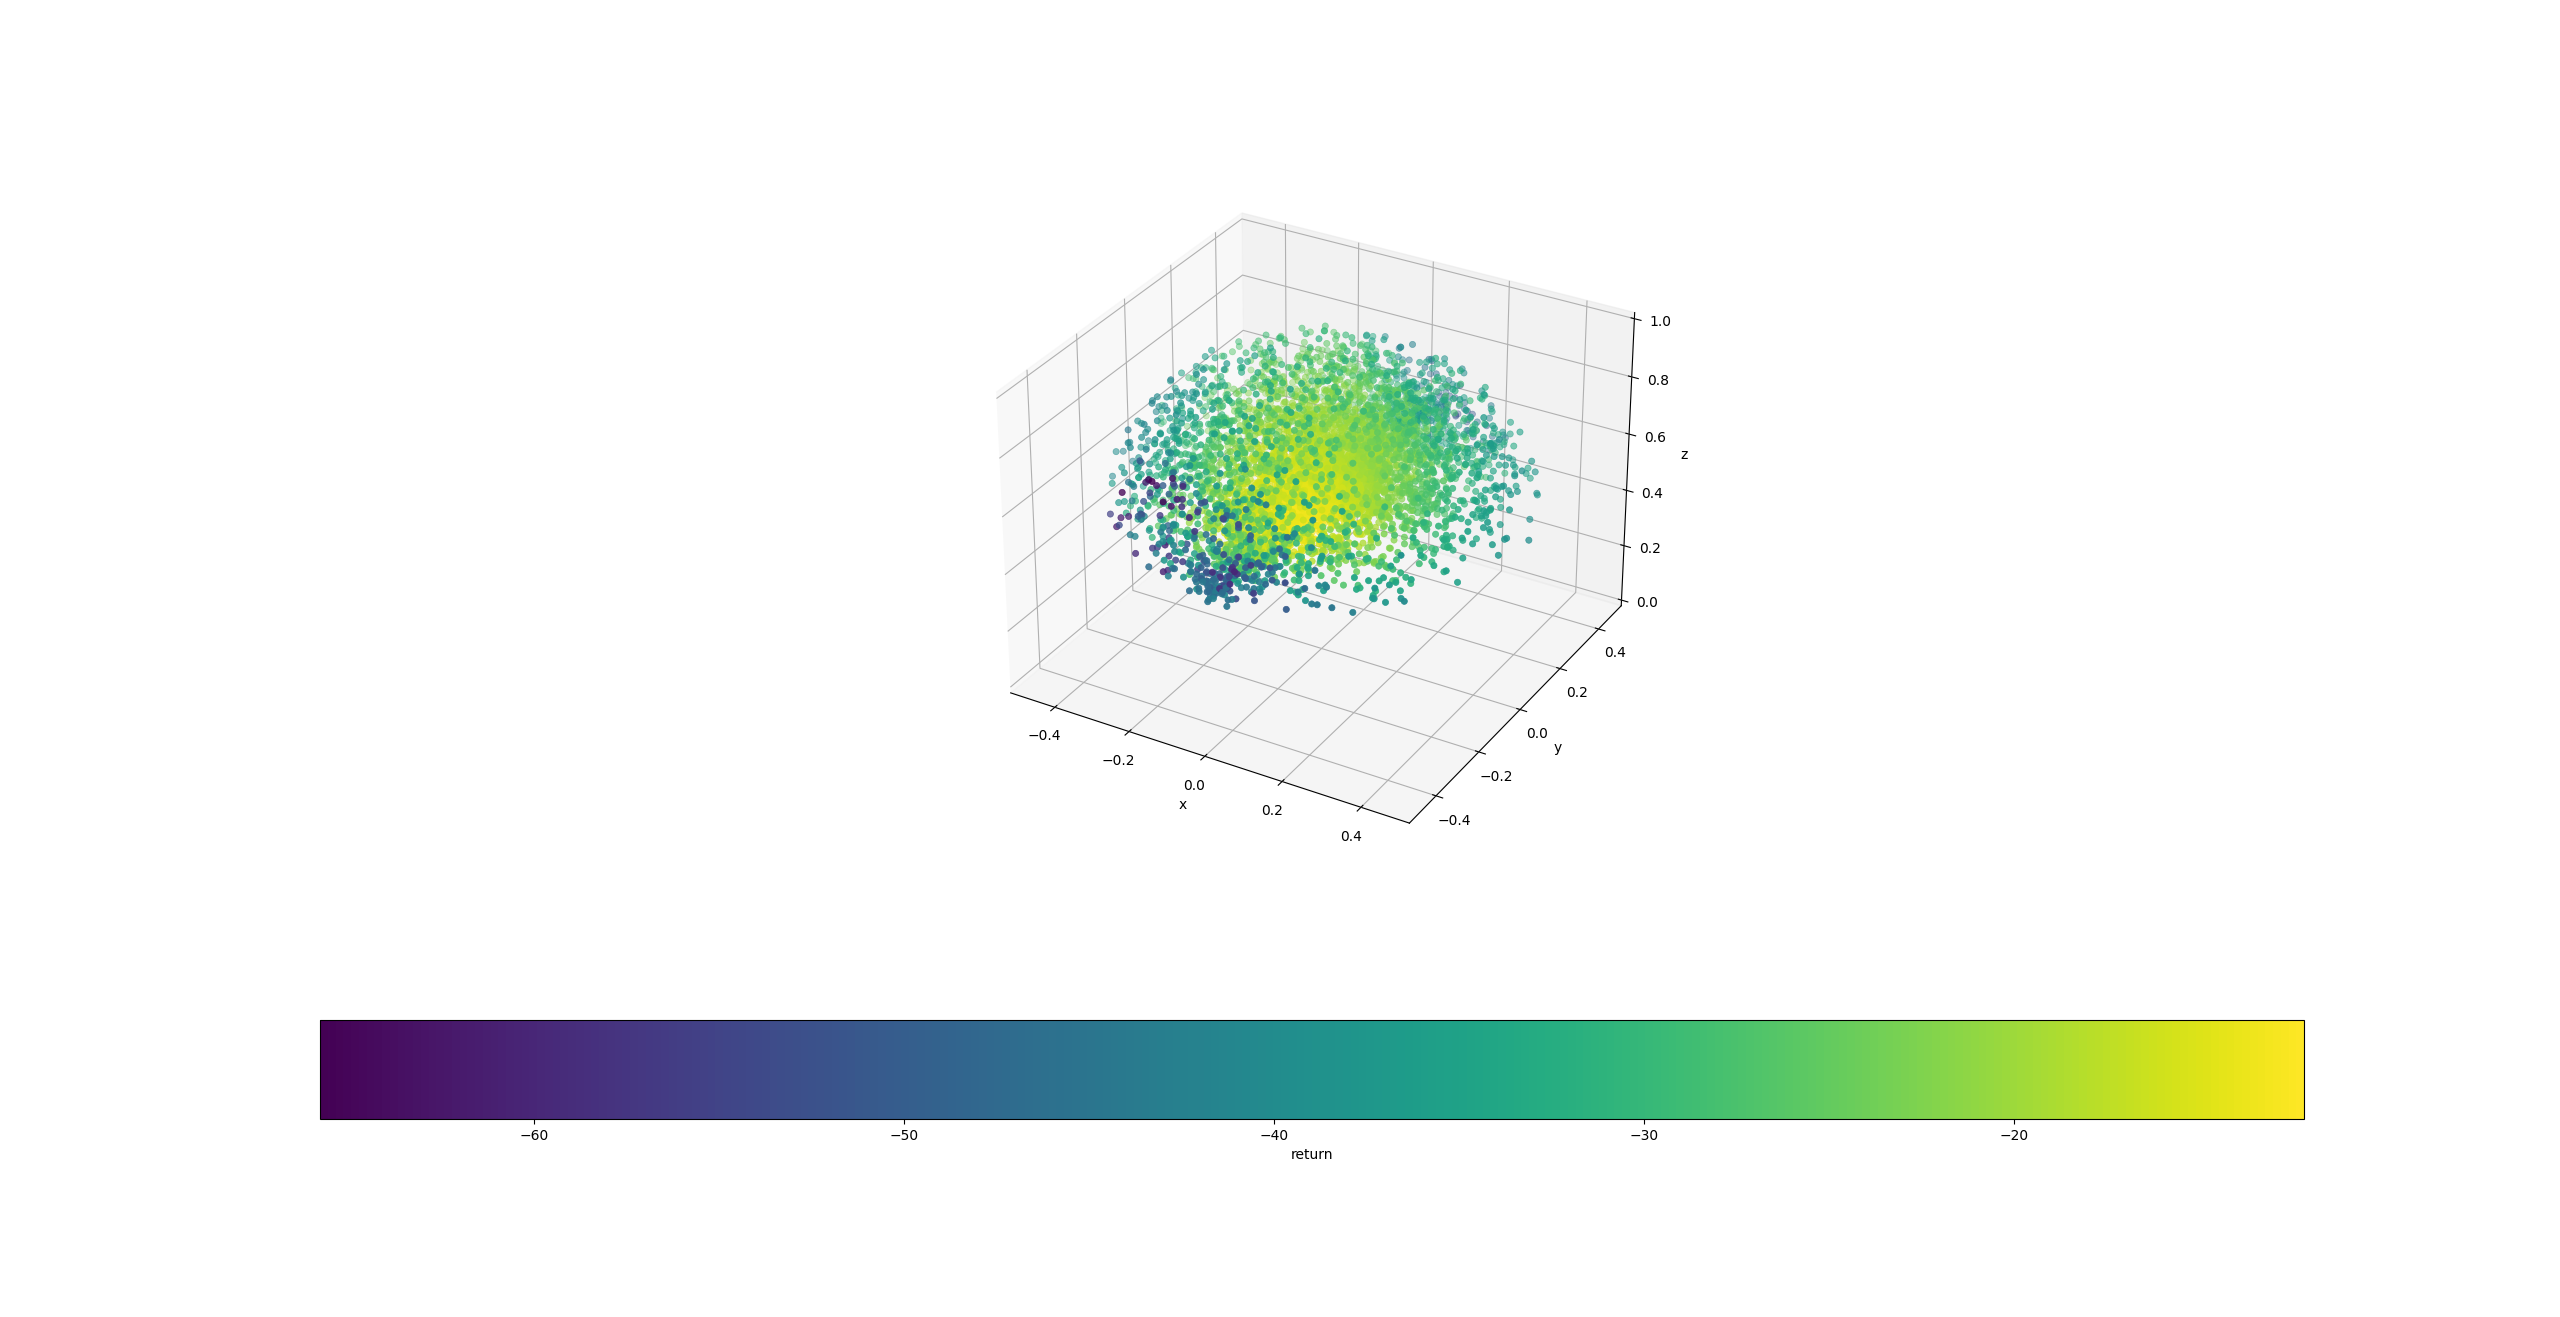
\includegraphics[width=\linewidth]{figures/potentialplot1.png}
	\caption{Expected Return of SAC policy for $7500$ random goals inside the 
	goal ball with a radius of $0.5m$}
	\label{fig:pot1}
\end{figure}

\begin{figure}
	\centering
	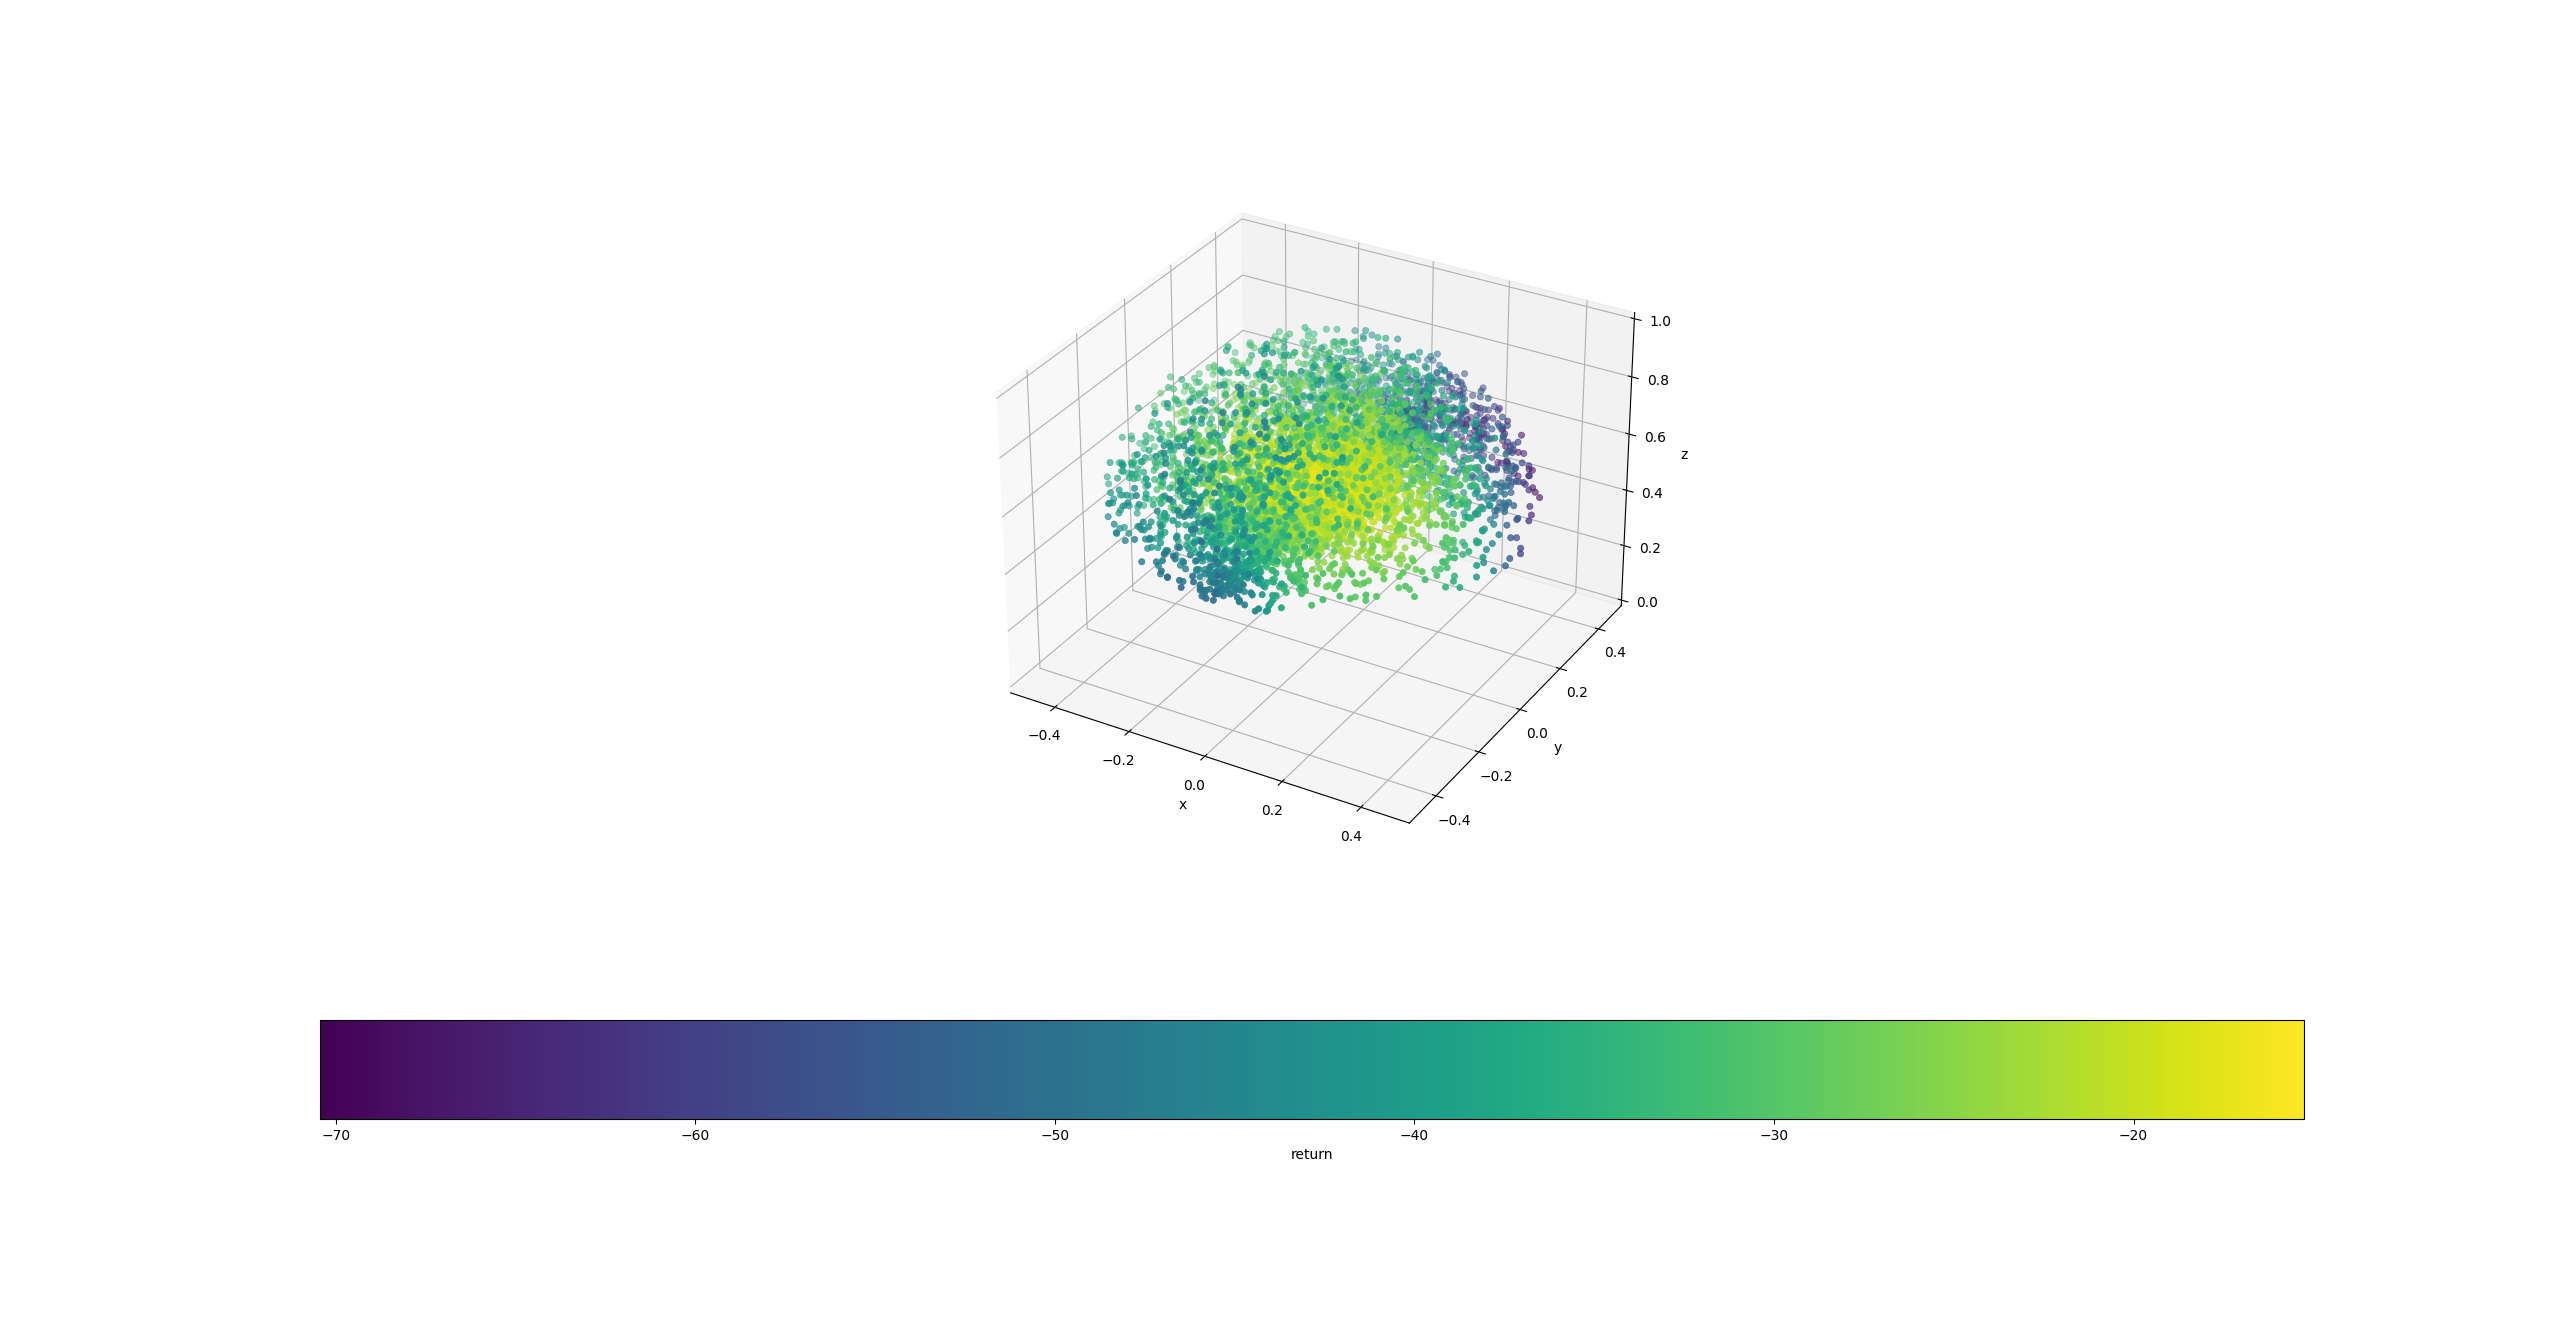
\includegraphics[width=\linewidth]{figures/potentialplot2.png}
	\caption{Expected Return of SAC policy with LCL ($\delta = 0.4$) for $7500$ random goals inside the 
	goal ball with a radius of $0.5m$}
	\label{fig:pot2}
\end{figure}

\begin{figure}
	\centering
	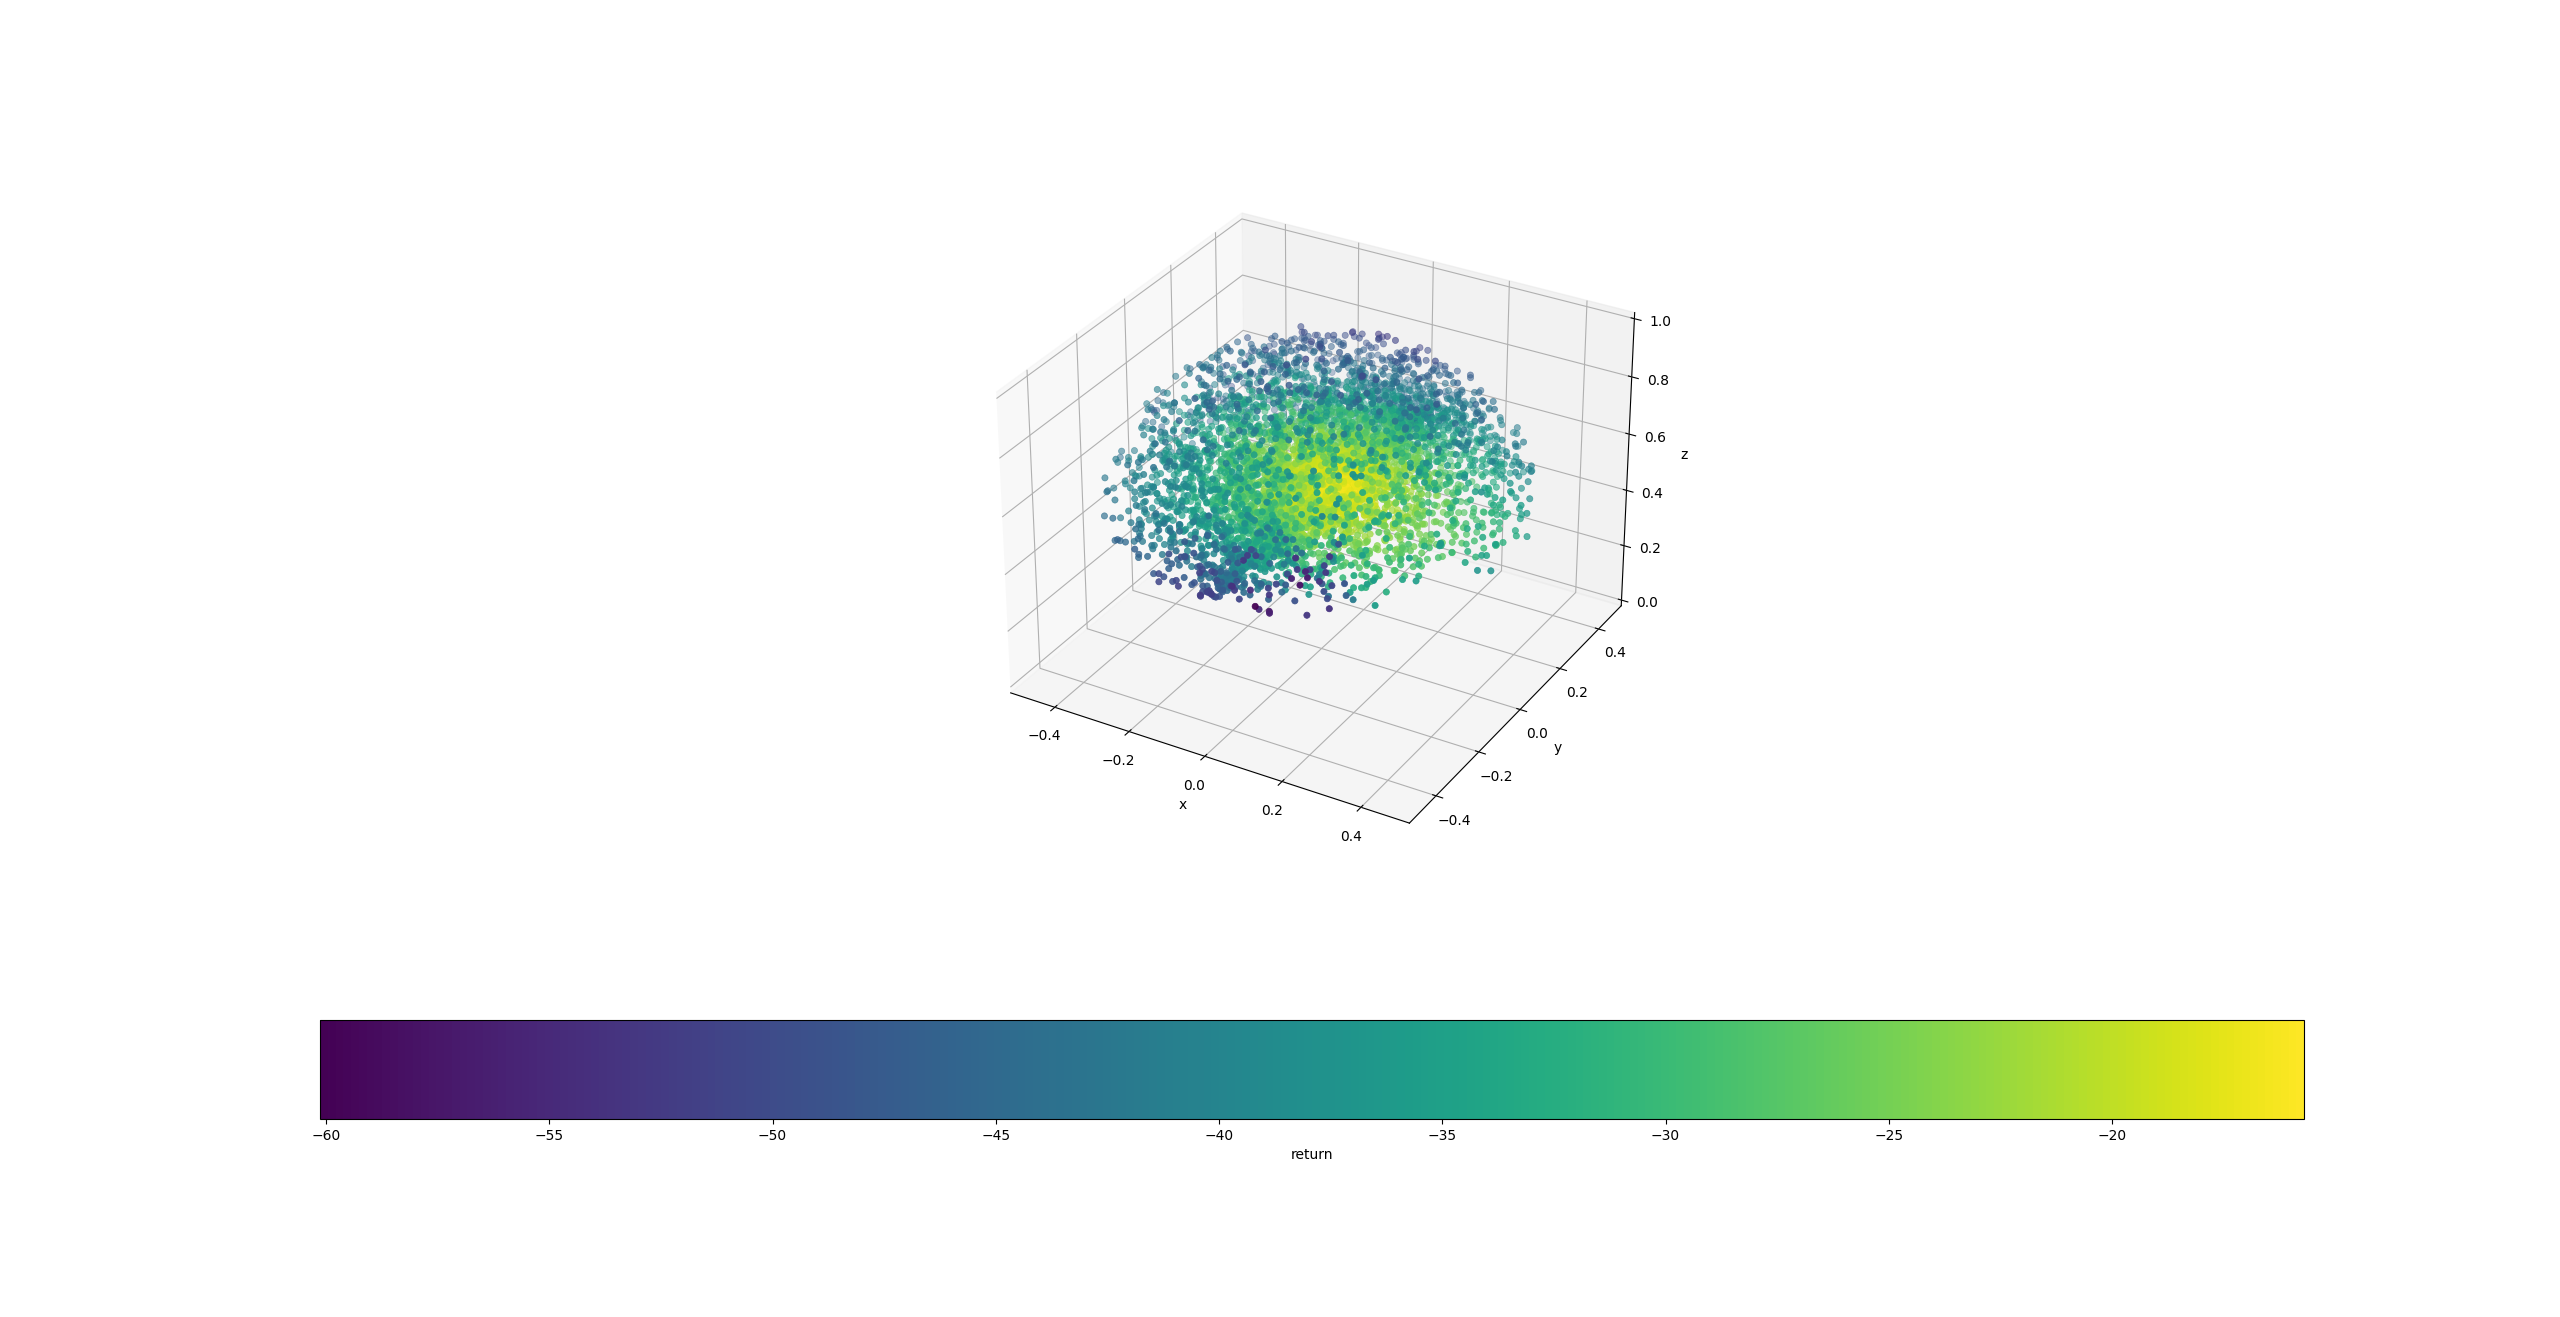
\includegraphics[width=\linewidth]{figures/potentialplot3.png}
	\caption{Expected Return of SAC policy with LCL ($\delta = 0.2$) for $7500$ random goals inside the 
	goal ball with a radius of $0.5m$}
	\label{fig:pot3}
\end{figure}

\begin{figure}
	\centering
	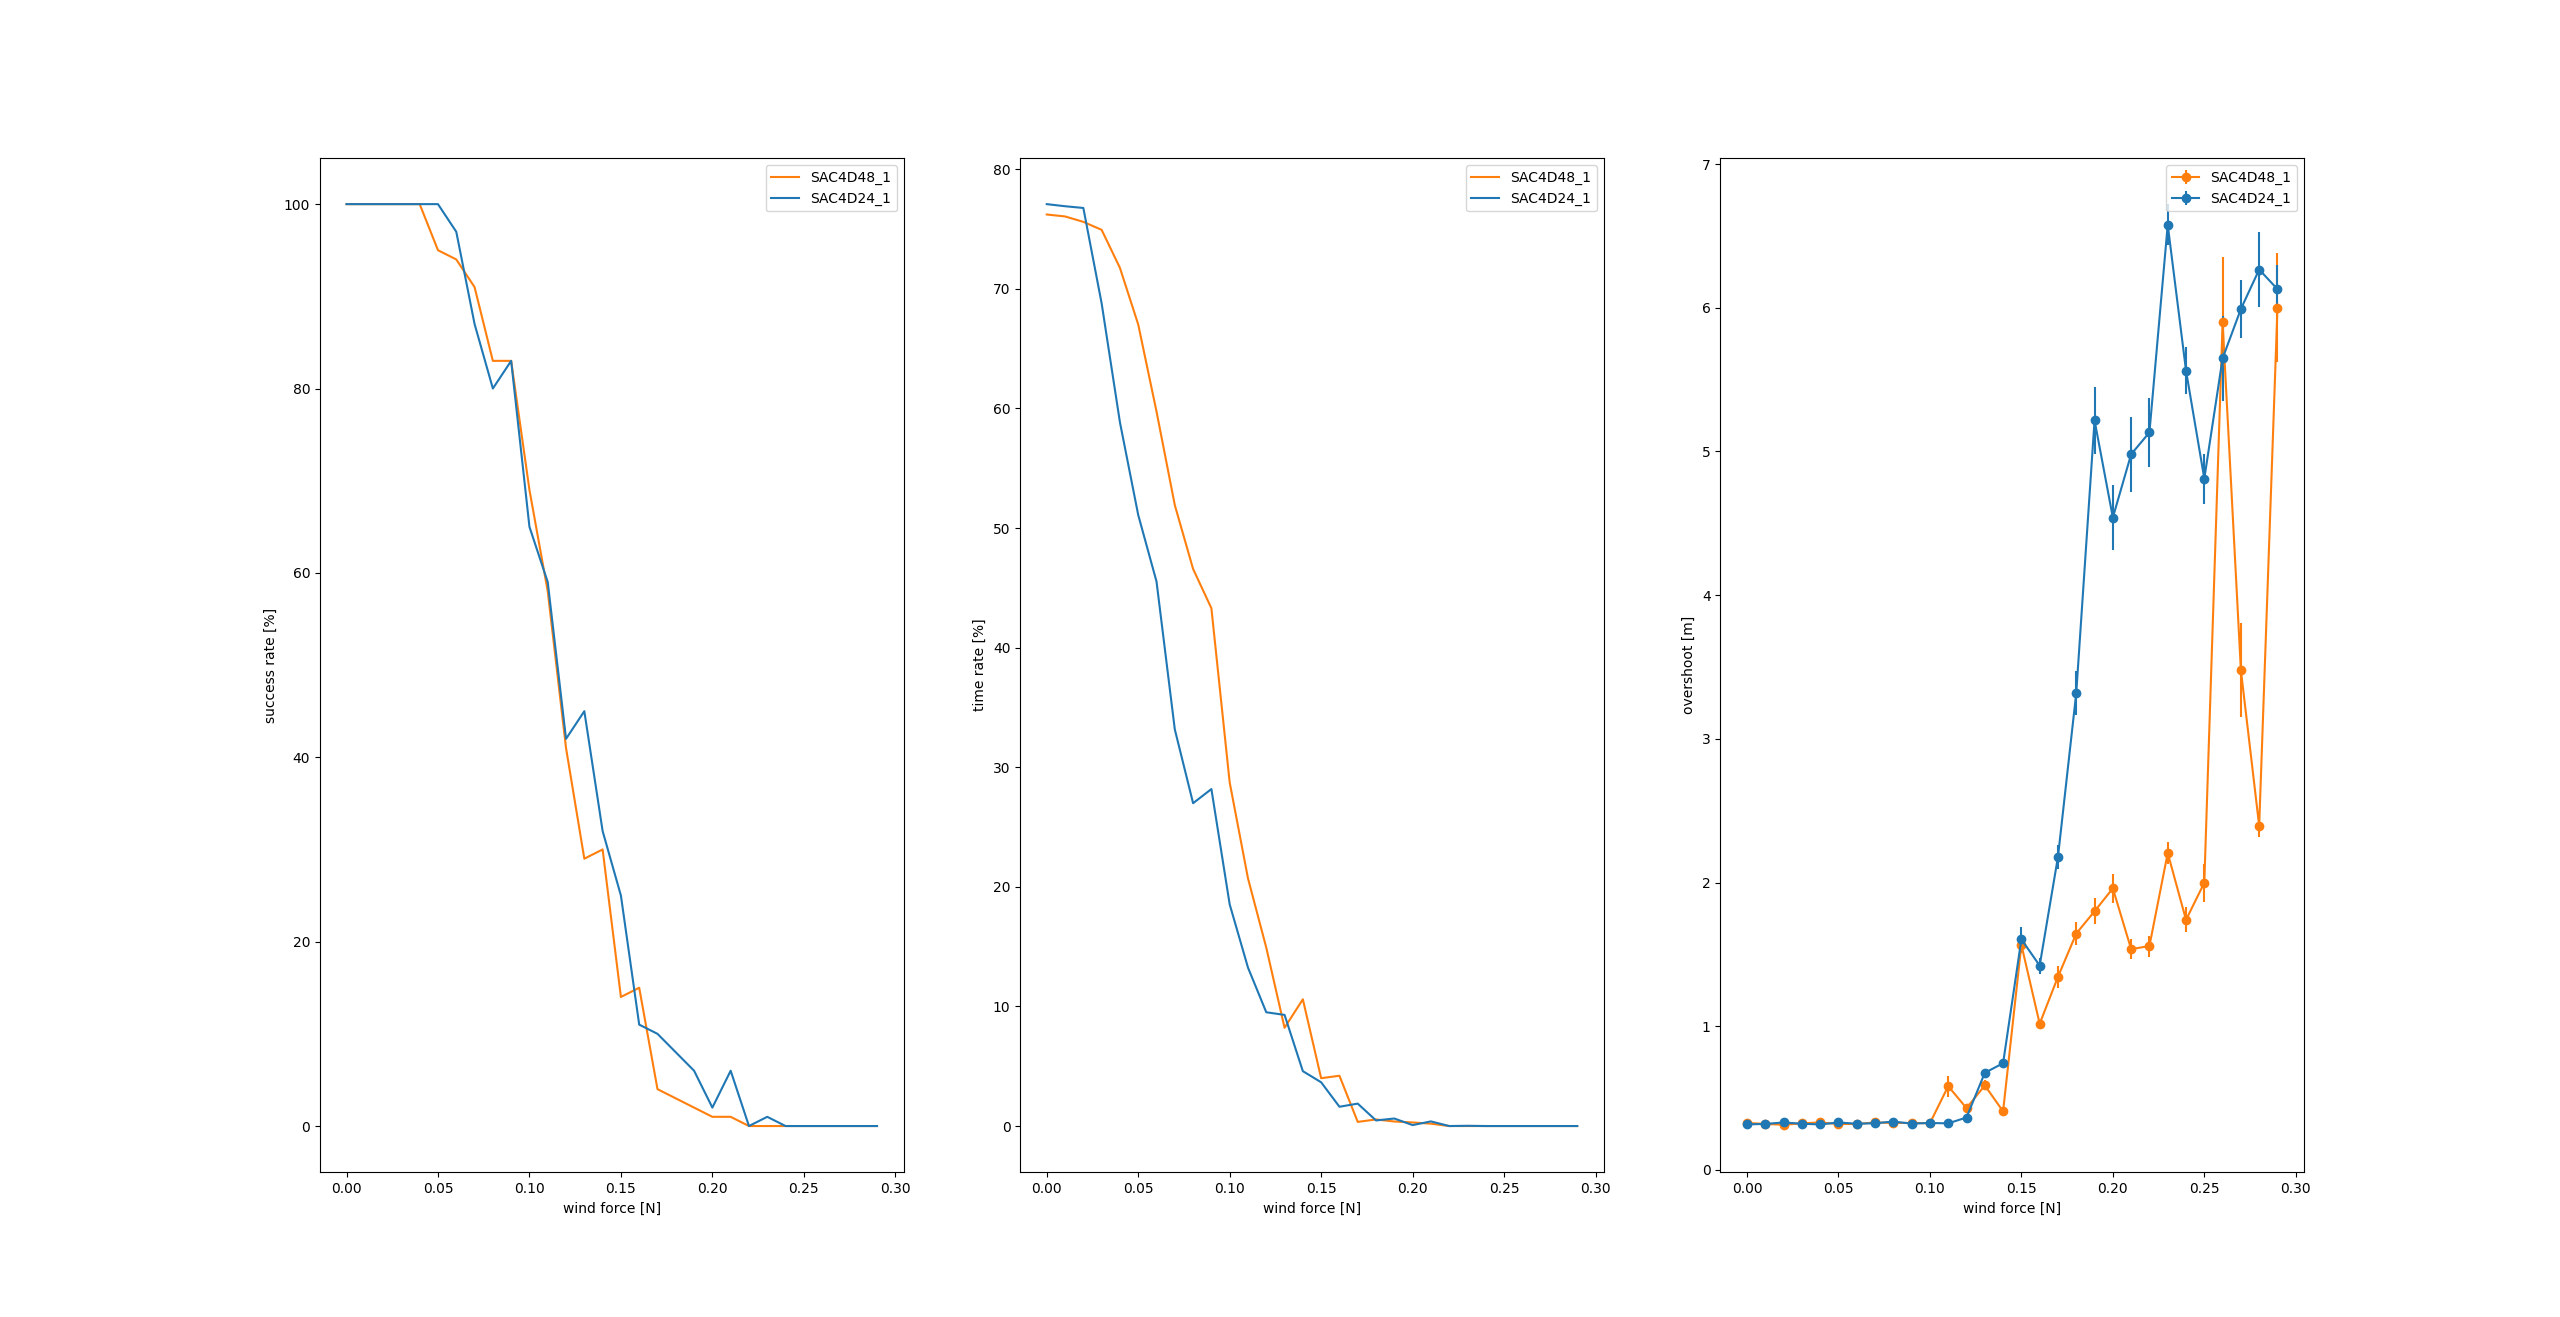
\includegraphics[width=\linewidth]{figures/windsuc.png}
	\caption{Success rate, time rate and overshoot $[m]$ with the associated standard error
	of SAC4D48 (orange) and SAC4D24 (blue) in a wind field of different strengths between $0N$ and $0.3N$}
	\label{fig:succ}
\end{figure}
